%%% This LaTeX source document can be used as the basis for your technical
%%% report. Intentionally stripped and simplified
%%% and commands should be adjusted for your particular paper - title, 
%%% author, citations, equations, etc.
% % Citations/references are in report.bib 

\documentclass[conference]{acmsiggraph}

\usepackage{graphicx}
\usepackage{float}
\graphicspath{{./images/}}
\newcommand{\figuremacroW}[4]{
	\begin{figure}[H] %[htbp]
		\centering
		\includegraphics[width=#4\columnwidth]{#1}
		\caption[#2]{\textbf{#2} - #3}
		\label{fig:#1}
	\end{figure}
}

\newcommand{\figuremacroF}[3]{
	\begin{figure}[H] % [htbp]
		\centering
		\includegraphics[width=#3\columnwidth]{#1}
		\caption[#2]{\textbf{#2}}
		\label{fig:#1}
	\end{figure}
}

\usepackage{lipsum}

\usepackage{xcolor}
\definecolor{lbcolor}{rgb}{0.98,0.98,0.98}
\usepackage{listings}

\lstset{
	escapeinside={/*@}{@*/},
	language=C,
	basicstyle=\fontsize{8.5}{12}\selectfont,
	numbers=left,
	numbersep=2pt,    
	xleftmargin=2pt,
	%numberstyle=\tiny,
	frame=tb,
	%frame=single,
	columns=fullflexible,
	showstringspaces=false,
	tabsize=4,
	keepspaces=true,
	showtabs=false,
	showspaces=false,
	%showstringspaces=true
	backgroundcolor=\color{lbcolor},
	morekeywords={inline,public,class,private,protected,struct},
	captionpos=t,
	lineskip=-0.4em,
	aboveskip=10pt,
	%belowskip=50pt,
	extendedchars=true,
	breaklines=true,
	prebreak = \raisebox{0ex}[0ex][0ex]{\ensuremath{\hookleftarrow}},
	keywordstyle=\color[rgb]{0,0,1},
	commentstyle=\color[rgb]{0.133,0.545,0.133},
	stringstyle=\color[rgb]{0.627,0.126,0.941},
}


\TOGonlineid{45678}
\TOGvolume{0}
\TOGnumber{0}
\TOGarticleDOI{1111111.2222222}
\TOGprojectURL{}
\TOGvideoURL{}
\TOGdataURL{}
\TOGcodeURL{}

\title{Development of an Android Guitar Tuner Application}

\author{Zoe Wall \\\ 40182161@live.napier.ac.uk \\
Edinburgh Napier University \\
Mobile Applications Development (SET08114)}
\pdfauthor{Zoe Wall}

\keywords{Android, fragments, accelerometer, file I/O, OpenGL}

\begin{document}

\teaser{
   \centering
   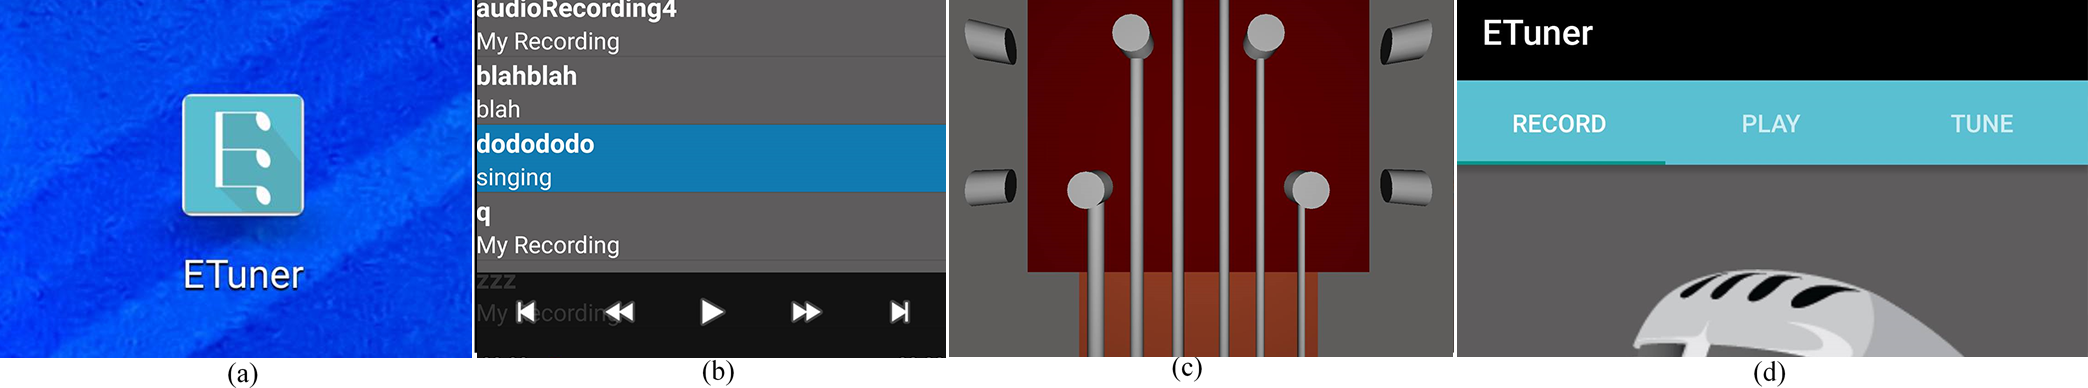
\includegraphics[width=1.0\textwidth]{images/teaser}
   \caption{Project screenshots. (a) Launch icon of Application, (b) Audio controller and clip selection, (c) 3D rendered guitar and (d) navigation tab bar.}
   \label{fig:teaser}
 }	

\maketitle

\begin{abstract} %% maybe change
This project aims to implement a mobile application prototype using the Android API. The application was intended to be a fully functional guitar tuner and audio recorder, also making use of the OpenGL API for embedded systems, to display 3D graphics. This report details the techniques used, and design decisions made within the development of the application.
\end{abstract}

\keywordlist
%\copyrightspace

\section{Introduction}

%%An introduction to your assignment stating its scope and content – this
%%should include a brief overview of your application choice and the
%%inspiration for your choice. Reference your reading. 
The requirements of this project were to develop a mobile application for the android platform. The initial ideas were that of a chromatic guitar tuner app. On the market at the moment there are hundreds of guitar tuner applications however the successful ones all seem quite similar. Reading an article about the best guitar tuner applications, they all seem to have the same design feel towards them. \cite{bestApps} Most are chromatic, meaning it 'recognizes each of the twelve chromatic (semitone) steps of the equal-tempered scale (C, C\#, D, D\#, E, F, F\#, G, G\# A, A\#, B)' which is useful as it can tune any instrument. \cite{Roland}

Most of them are very complex, with many different features such as chord libraries and metronomes. Hardly any application within the top ten has a reference pitch section, and if they do, it's is almost always an extra feature. Making a decision to use a reference tuner as a main feature of the project would make the application unique compared to the hundreds of tuner applications already on the App Store.

Another unique feature that was planned to implement would be that of a voice recorder and play back function. Taking inspiration from these successful applications, for this project it was decided to incorporate an extra feature, that would use more elements of the API to fit with the project's specifications. A voice recorder is a tool used by many singer-songwriters to quickly sing or strum down a tune or melody for later reference. However, none of the researched guitar applications included this as a feature. Most devices come with their own voice recorder applications built-in however from experience, the recordings are usually difficult to edit, find or delete. Which inspired the project to include a very simple user interface where the user can in one tap discard the recording immediately, or if they wish give it a more meaningful name than "Voice0001" for example.  

\subsection{Related Work}

\paragraph{DaTuner} One app that is very simple and particularly useful is the DaTuner. The free version of the application is very quick and simple to use, however if a user was looking for more, they will also find some advanced features within the pro version (see figure \ref{fig:daTune}). DaTuner is a good application as it is very quick to use, it launches straight into a tuner which you can use automatically without any set-up or navigation.

\figuremacroW
{daTune}
{Screenshot of a simple chromatic tuner - DaTuner. Note how clear the complex information is displayed through a simple two-colour display.}
{\protect\cite{DaTune}}
{1.0}

\paragraph{Martin Guitar Tuner} Another application that is inspirational is the C.F. Martin \& Co. Guitar Tuner App (see Figure \ref{fig:martinTuner}). Overall it is not a very good application, it's uses a "hamburger" style navigation menu and it's tuner pages are low-quality images with very little user interaction. Hamburger menus, even though widely used, are not a good way of displaying menu items. They are useful in the sense that complex navigation can be hidden behind a button which saves screen space, but they are 'less efficient' due to the need of tapping the button before you can reach any options. They also make the ability to glance at an available interaction more difficult, which can lead to users forgetting that some features exist. \cite{hamburger} One good thing about the application is that it includes a very basic approach to an ear tuner. It is simple, you tap the tuning peg and the corresponding note plays, which is why it is inspiring. For this project, the reference tuner will be implemented using a 3D rendered guitar with animation to show the user which string is being played.

\figuremacroW
{martinTuner}
{Screenshot of the Martin Guitar Tuner. Note the inclusion of a reference note tuner.}
{\protect\cite{Martin}}
{1.0}

\paragraph{Samsung Galaxy S6 Voice Recorder}

Taking inspiration from the pre-installed Voice Recorder application from the Samsung Galaxy S6 device, an aim for the voice recorder tab is to have instant avalible playback functionality.

\section{Software Design}

\subsection{Design Decisions}

A decision was made to favour a more simple app than some of the more feature-heavy application. This was due to the similarities of most applications already on the market, one of the project aims was to produce something different however still useful. The aim was to develop an application to be used as an everyday tool and not as a game or distraction.

When researching implementation of chromatic tuning software, it seemed a little beyond the scope of the assignment. The biggest issue with the implementation was the pitch detection. On first glance, it can seem as easy as putting data into a FFT, Fast-Fourier Transform. A FFT, is an algorithm that can compute compromising frequencies of a given signal. \cite{FFT} However, it also requires some pre-processing of the sampled data. For this project, it was inappropriate as the objectives of the tasks were to develop an application that used advanced features of the android API, so it was decided that implementing a pitch detection feature wouldn't have met these objectives. Instead, it was decided to include a reference note tuner implemented with 3D graphics.

%%graphics

As the focus of the project was using the android API, it was decided that the app should include a recording and playback feature. The implementation of a simple voice recorder. %% something to do with the app wanting to 

EXPLAIN WHY THIS SHOWS OFF THE API

%% story board
%% wireframe
%% asking guitarist what they wanted 

\subsection{Experience Story}

"A guitarist is walking in the park, an idea occurs to him of a melody. He opens the application, presses record and starts singing. He wants to remember this idea for when he arrives home. He stops the recording and can quickly decide if he wants to discard it or rename the file and save it. He types the name "In the Park" taps save, he swipes right and can playback his recording instantly by tapping on it's name within the view." 

In creating an experience story for a particular scenario. %% Read notes on PID

\subsection{User Interface Sketches}

\figuremacroF
{playSketch}
{A quick sketch of a user interface design for the play tab.}
{1.0}

\figuremacroF
{recordSketch}
{A quick sketch of a user interface design for the record tab.}
{1.0}

\figuremacroF
{tuneSketch}
{A quick sketch of a user interface design for the tune tab.}
{1.0}

SWIPE VIEWS!!
http://developer.android.com/design/patterns/swipe-views.html

\subsection{Activity Diagrams}

After completing rough sketches of the user interface design. The application was split into three tabs and activity diagrams were drawn to model the software. Figures \ref{fig:RecordTab}, \ref{fig:PlayTab} and \ref{TuneTab} show the high-level activity diagrams created for the Recording tab, the Play tab and the Tune tab respectively.

These were key to the design of the implementation as they showed a structured flow of control for the program. Lower-level models could have been drawn with functional decomposition, however these diagrams were sufficient to begin implementation due to the main requirements and logic of the application being included.

\figuremacroF
{RecordTab}
{The activity diagram for the Record Tab}
{1.0}

\figuremacroF
{PlayTab}
{The activity diagram for the Play Tab}
{1.0}

\figuremacroF
{TuneTab}
{The activity diagram for the Tune Tab}
{1.0}
 
\section{Implementation}

\subsection{Navigation}

For the main navigation of the app, one main activity was used alongside fragments. In doing so, a tab layout could be used making it easy for the user to see what options are available. (See Figure \ref{fig:navBar}) To implement this, a ViewPager and custom PagerAdapter was used. A ViewPager does not pause fragments that are next to the visible tab to allow for smoother scrolling.

\figuremacroF
{navBar}
{An image of the final implementation of the navigation bar. It consists of the title of the application and three tabs which are clickable or swipeable.}
{1.0}

For the implementation, the PagerAdapter created extended the FragmentStatePagerAdapter class of the API. It was chosen due to the fact it "It destroys fragments as the user navigates to other pages, minimizing memory usage." \cite{Swipe} This meant that if the record tab was visible, the tune tab would call it's onPause lifecycle method, stopping the continuous call for the renderer's update function.

\subsection{Recording}

The recording fragment of the app uses a MediaRecorder to save an audio recording in AAC format. Most built in voice recorder applications on mobile phones don't allow for customisation of the media file's meta data. From the experience story, an aim of the project was to implement a function to quickly change the file name, add a description and be able to playback showing these values. Without using an external library, editing meta data for recorded files was difficult. It could have been done using ID3Tags however the android library does not support encoding for MP3. \cite{SupportedMedia} To work around this, android's MediaStore was used.

The MediaStore is a content provider that contains meta data for all available media on both external and internal storage of the device, similar to an SQL database. When adding or removing media from a device, the meta data stored remains until Android scans the system for new media. Typically this happens when the device is booted, however it can be called explicitly by broadcasting an Intent. \cite{MediaStore} Therefore when an audio file was recorded and saved, a function was used to insert this into the database, see Listing \ref{lst:insertDB}.

%%\begin{minipage}{\linewidth}

\begin{lstlisting}[label = {lst:insertDB}, caption={Inserting File into MediaStore Database}]
public void insertFileIntoDatabase(String fileName, String fileDesc)
{
    File mySound = new File(recDir, fileName + fileExt);
    	
    // rename file
    boolean rename = tempFile.renameTo(mySound);
    	
   	// add recording to media database
   	ContentValues values = new ContentValues(4);
   	long current = System.currentTimeMillis();
   	values.put(MediaStore.Audio.Media.TITLE, fileName);
   	values.put(MediaStore.Audio.Media.ARTIST, fileDesc);
   	values.put(MediaStore.Audio.Media.ALBUM, albumName);
   	values.put(MediaStore.Audio.Media.DATE_ADDED, (int) (current / 1000));
    values.put(MediaStore.Audio.Media.MIME_TYPE, "audio/AAC");
   	values.put(MediaStore.Audio.Media.DATA, mySound.getAbsolutePath());
    	
   	ContentResolver contentResolver = TabSwitcher.getmContext().getContentResolver();
    	
   	Uri base = MediaStore.Audio.Media.EXTERNAL_CONTENT_URI;
   	Uri newUri = contentResolver.insert(base, values);
    	
   	TabSwitcher.getmContext().sendBroadcast(new Intent(Intent.ACTION_MEDIA_SCANNER_SCAN_FILE, newUri));
   	
   	Toast.makeText(TabSwitcher.getmContext(), "Added File " + fileName, Toast.LENGTH_LONG).show();
    	
   	// sets dirty flag for updating list from database
   	TabSwitcher.setListDirty(true);
}
\end{lstlisting}

To save resources, a recording is initially stored with a temporary file name so if the user decides not to keep the recording, they can easily just click delete and try again. Once a user clicks save, the file is renamed.

To insert meta data into the database, see the method used on line 21 of Listing \ref{lst:insertDB}. This inserts a row into a table at the given URL, with the relevant ContentValues. For the description of the file, the Artist's column was used, as there was no option, without creating a separate database to customise the columns. In using the MediaStore as opposed to a 3rd party library to create meta data for the recordings, it means that they can also be accessed by any other app on the system.

Finally, the intent was broadcast to the MediaScanner and a static flag was set, so that the play tab can update the list of files and show the new recording when navigated to.

In keeping with the proposed graphic design, the layout of the tab was filled with a vector graphic of a microphone with a free to use license. \cite{microphone} It also included an image button with a record icon created for the project.

\figuremacroF
{PlayTabSS}
{A screenshot of the final implementation of the record tab. The button at the bottom switches from a record icon to a stop icon when pressed to indicate the app is recording.}
{1.0}

Once the recording is stopped, a custom alert dialog was used to allow the user to delete the file, or save their own details. To stop the dialog closing if an invalid file name was entered, the click event handlers were created and then overridden, see Figure \ref{fig:dialog}

\figuremacroF
{dialog}
{A screenshot of the alert dialog that is used when a user stops a recording. Note the toast that appears if the filename is already in use.}
{1.0}

\subsection{Playback}

For the playback implementation, a class was created to store audio clip objects. Each contained an ID, a title and an artist. This meant that when the fragment is created, the device is queried for all audio content stored. Due to the fact, the album was set as constant for every recorded file meant that only files with the exact album name were initialised as Audio Clip objects, see Listing \ref{lst:query}.

\begin{lstlisting}[label = {lst:query}, caption={Conditional Statement for Creating Audio Clips}]
if (soundCursor.getString(albumColumn).equals(Recorder.albumName))
{
	clipList.add(new AudioClip(thisId, thisTitle, thisArtist));
}
\end{lstlisting}

By using an ArrayList container to store these AudioClip objects, the List View within the Fragment's layout can be populated by using a custom Adapter class. This means that for every object in the list, the adapter can easily iterate through the list retrieving each of the instance variables and setting the appropriate text views to display the information. Rather than having to query the database each time, when the play tab becomes visible, it checks whether the flag set in the record tab is true, if so, it will clear the list and re-populate it. 

\figuremacroF
{playback}
{An image of the final implementation of the Play tab. It uses Android's own MediaController to control the play functions, and highlights the current chosen track.}
{1.0}

For the playback of these audio clips, a sound Service was implemented meaning that if the user wanted, they could continue listening to their audio clips if they have navigated away from the application, or if they lock their device. Playback was controlled through an instance of a MediaPlayer that was bound to the Service, and a default MediaController for the user interface. As the project focus was more on the guitar tuner and recording aspect, it seemed inappropriate to redesign a media controller just for this purpose, the implementation of this can be seen in Figure \ref{fig:playback}.

\subsection{Tuning}

For implementation of the tuning tab, a Frame Layout containing a SurfaceView was used. This SurfaceView was inflated using a custom OpenGL context which rendered to the screen. \cite{OpenGL}

NEED TO TALK ABOUT ACCELEROMETER HERE


\section{Evaluation}
%%4. An evaluation of your implementation. Points to consider discussing in this section are:
%%• A comparison against the original concept as detailed in your introduction
%%• Comparison against other applications/games in the genre, particularly the ones that inspired your choice
%%• An evaluation of your app against user feedback or as compared with other apps/ games
%%• Possible improvements to your application

The original concept as outlined in my introduction was to develop a guitar tuner application that was unique compared to the ones already available on the market. This was to include a reference tuner and a voice recorder function. The final application developed implements both these features with full functionality. 

Similarly to the DaTuner application, a simple colour scheme was used, and remains consistent throughout. However, processing sound input through a chromatic tuner was too advanced for the project and was not implemented. The developed application is also very quick and simple to use, much like this app.

The application developed encompasses the reference tuner inspired by the Martin Guitar Tuner, however it improves a lot on the user experience design by incorporating simple lateral navigation using a swipe-able tab view. This by far is easier to use than the "hamburger" style menu of the Martin Guitar Tuner, because it allows the user to see every option available to them instantly, and to navigate between them within one movement. Even though, the ability to tap on a sound and have it play is a good feature of the Martin app that is not implemented within this project, the developed application improves on the feedback of this particular reference tuner as of the added functionality of the looping play-back. When tuning a guitar by ear, looping play back is often essential to ensure the tone is correct. The inclusion of this feature allows the user to continuously play the tone whilst attempting to tune their guitar - without having to repeatedly interact with the device.

%% voice recorder
%% user feedback

\subsection{Further Work}

In improving the application, the next steps are to build more functionality in the app by including a chromatic tuner. 

One improvement to be made to the application is refinement of the user interaction for the Tune tab. Currently, the only way to change the chosen string is to shake the device, this is a unique feature that shows of the use of the Android API however it is limited. Implementing functionality where a user can tap on one of the strings or tuning pegs, similar to the Martin Guitar Tuner, would be a nice addition to the applications user interface. However, due to the fact the surface view is implemented using OpenGL ES, it means that to make this possible calculations would have to be made on the exact position of the object within the 3D space. This is called picking, which is a form of ray casting. \cite{ray} A bounding volume would have to be calculated for each clickable object within the scene, and each time the user would tap on the screen calculations must be performed to see if the ray, from the screen coordinates, intersects with the bounding volume of the shape. This was definitely beyond the scope of the project's requirements, as it ventures on more computer graphics than mobile app development, however if implemented would improve the application significantly. As for the current shaking implementation, it is not very accurate and could be improved.

Aesthetics wise, the tune tab could also be improved by loading in a model of a guitar headstock to make it look more realistic. This was originally going to be the case, however a suitable model could not be found, with separate strings. Another way of making the guitar more realistic would be to change the string vibration animation to use vertex displacement within the shader program. Currently the shader program only shades each pixel according to the lighting model. However, a separate shader program could be written to change the actual geometry of the strings and displace it's vertices along a sine wave, modelling an actual guitar string's movement.

\section{Summary}

%% CONCLUSION

The only resources used that were not created for this project include the vector graphic of the microphone \cite{microphone}, and the reference notes \cite{refNotes}.

Any online tutorials used for reference for parts of the Android API that were not covered in the module are below:
\begin{itemize}
	\item %% STUFF HERE
\end{itemize}


\bibliographystyle{acmsiggraph}
\bibliography{report}


\end{document}